\documentclass{beamer}

\newenvironment{tightcenter}{%
  \setlength\topsep{0pt}
  \setlength\parskip{0pt}
  \begin{center}
}{%
  \end{center}
}

\usepackage[polish]{babel}
\usepackage{chessfss}
\usepackage{hyperref}
\usepackage{qtree}
\usepackage{mathtools}
\usepackage{dirtytalk}
\usepackage{epigraph}
\usepackage{textgreek}
\usepackage[utf8]{inputenc}
\usepackage{times}
\usepackage[T1]{fontenc}
\usepackage{tikz}
\usepackage{csquotes}
\usepackage{amsmath}
\usepackage{fancyvrb}
\usepackage{ulem}
\usepackage{adjustbox}

\newenvironment{Snippet}{\Verbatim[samepage=true]}{\endVerbatim}

\newcommand{\soutthick}[1]{%
    \renewcommand{\ULthickness}{2.4pt}%
       \sout{#1}%
    \renewcommand{\ULthickness}{.4pt}% Resetting to ulem default
}

\usetheme{Pittsburgh}

\usecolortheme{owl}

% \title{What I want from a coding tool}

\author{Panicz Maciej Godek}

\institute{
  \tiny{\href{mailto:godek.maciek@gmail.com}{\textbf{godek.maciek@gmail.com}}}
}

\date{04.10.2024}

\begin{document}

\begin{frame}[plain]
  \begin{center}
    {\huge What I want from a coding tool} \\*
    {\huge \phantom{-----What is programming?}}
  \end{center}
\end{frame}

\begin{frame}[plain]
  \begin{center}
    {\huge What I want from a \soutthick{coding} tool} \\*
    {\huge \phantom{-----What is programming?}}
  \end{center}
\end{frame}

\begin{frame}[plain]
  \begin{center}
    {\huge What I want from a \soutthick{coding} tool} \\*
    {\huge \phantom{-----What is} programming\phantom{?}}
  \end{center}
\end{frame}

\begin{frame}[plain]
  \begin{center}
    {\huge \phantom{What I want from a coding tool}} \\*
    {\huge \phantom{-----}What is programming?}
  \end{center}
\end{frame}


{ % all template changes are local to this group.
  \setbeamertemplate{navigation symbols}{}
  \begin{frame}[plain]
    \begin{tikzpicture}[remember picture,overlay]
      \node[at=(current page.center)] {
        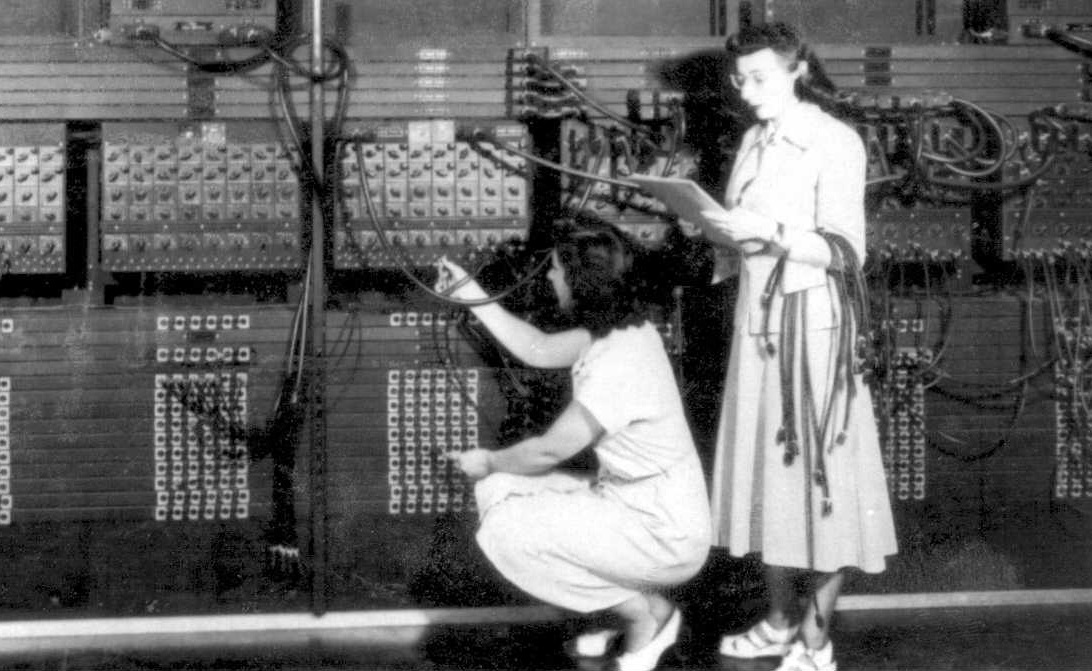
\includegraphics[height=\paperheight]{eniac1.jpg}
      };
    \end{tikzpicture}
  \end{frame}
}

{ % all template changes are local to this group.
  \setbeamertemplate{navigation symbols}{}
  \begin{frame}[plain]
    \begin{tikzpicture}[remember picture,overlay]
      \node[at=(current page.center)] {
        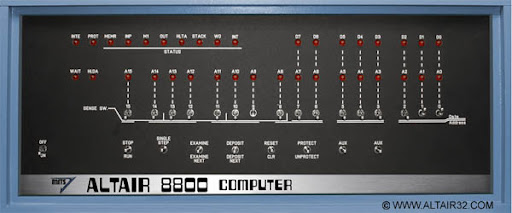
\includegraphics[width=\paperwidth]{altair8800.jpg}
      };
    \end{tikzpicture}
  \end{frame}
}


{ % all template changes are local to this group.
  \setbeamertemplate{navigation symbols}{}
  \begin{frame}[plain]
    \begin{tikzpicture}[remember picture,overlay]
      \node[at=(current page.center)] {
        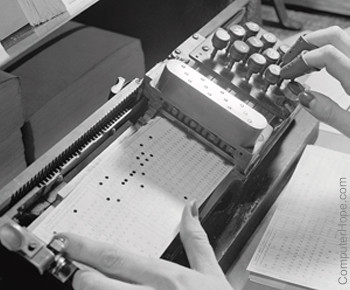
\includegraphics[width=\paperwidth]{punch-card-machine.jpg}
      };
    \end{tikzpicture}
  \end{frame}
}

{ % all template changes are local to this group.
  \setbeamertemplate{navigation symbols}{}
  \begin{frame}[plain]
    \begin{tikzpicture}[remember picture,overlay]
      \node[at=(current page.center)] {
        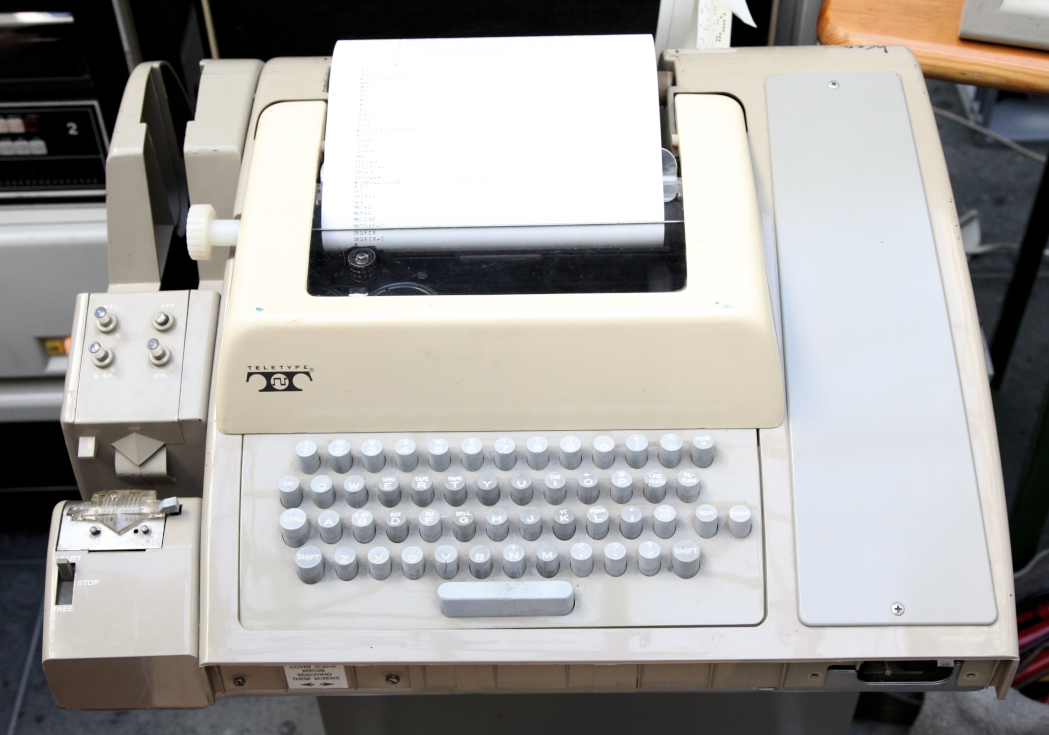
\includegraphics[width=\paperwidth]{Teletype.jpg}
      };
    \end{tikzpicture}
  \end{frame}
}

\begin{frame}[plain]
  \begin{center}
    {\huge Is programming \textit{making computers do things?}}
  \end{center}
\end{frame}

{ % all template changes are local to this group.
  \setbeamertemplate{navigation symbols}{}
  \begin{frame}[plain]
    \begin{tikzpicture}[remember picture,overlay]
      \node[at=(current page.center)] {
        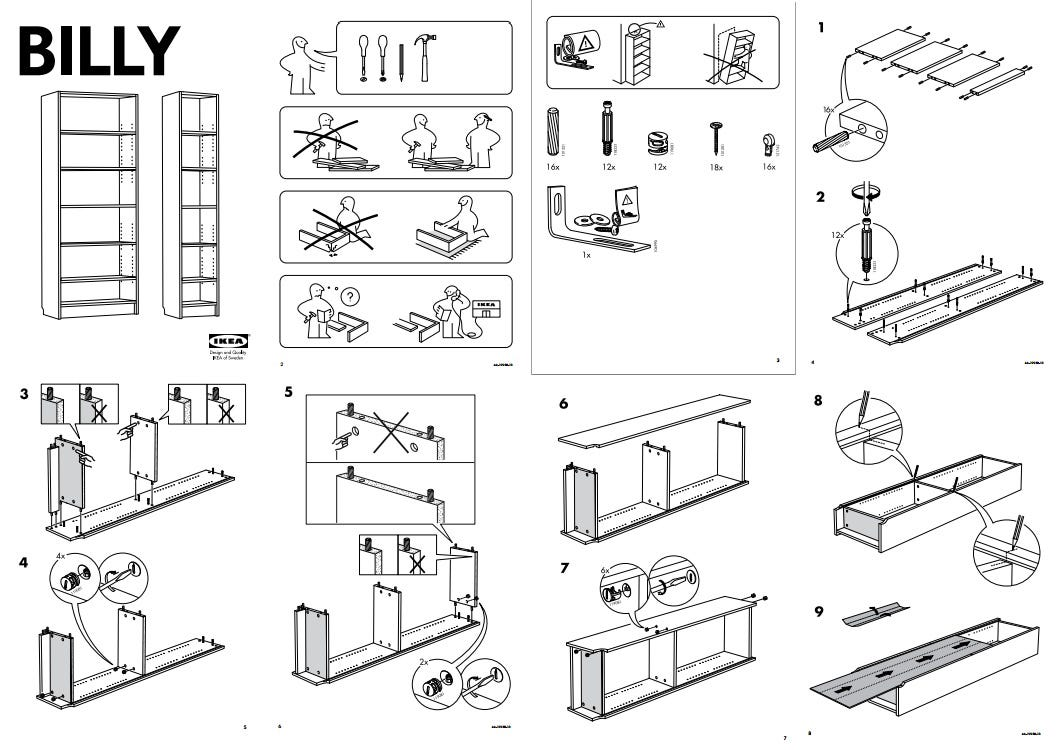
\includegraphics[width=\paperwidth]{ikea.jpg}
      };
    \end{tikzpicture}
  \end{frame}
}

{ % all template changes are local to this group.
  \setbeamertemplate{navigation symbols}{}
  \begin{frame}[plain]
    \begin{tikzpicture}[remember picture,overlay]
      \node[at=(current page.center)] {
        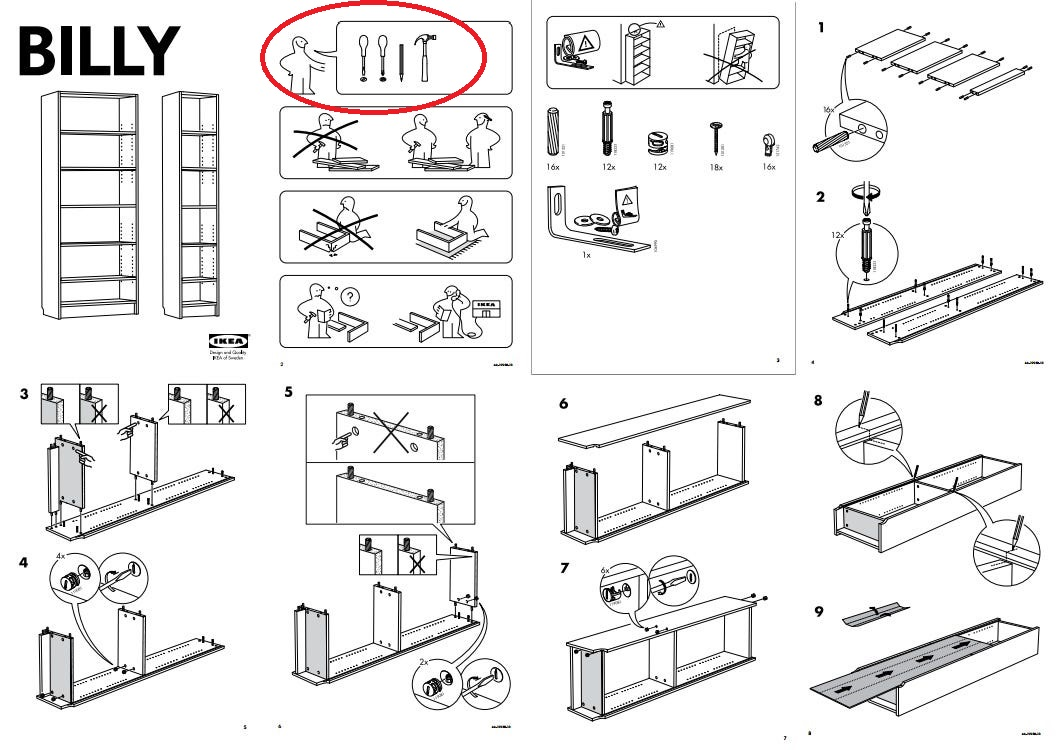
\includegraphics[width=\paperwidth]{ikea-utils.jpg}
      };
    \end{tikzpicture}
  \end{frame}
}

{ % all template changes are local to this group.
  \setbeamertemplate{navigation symbols}{}
  \begin{frame}[plain]
    \begin{tikzpicture}[remember picture,overlay]
      \node[at=(current page.center)] {
        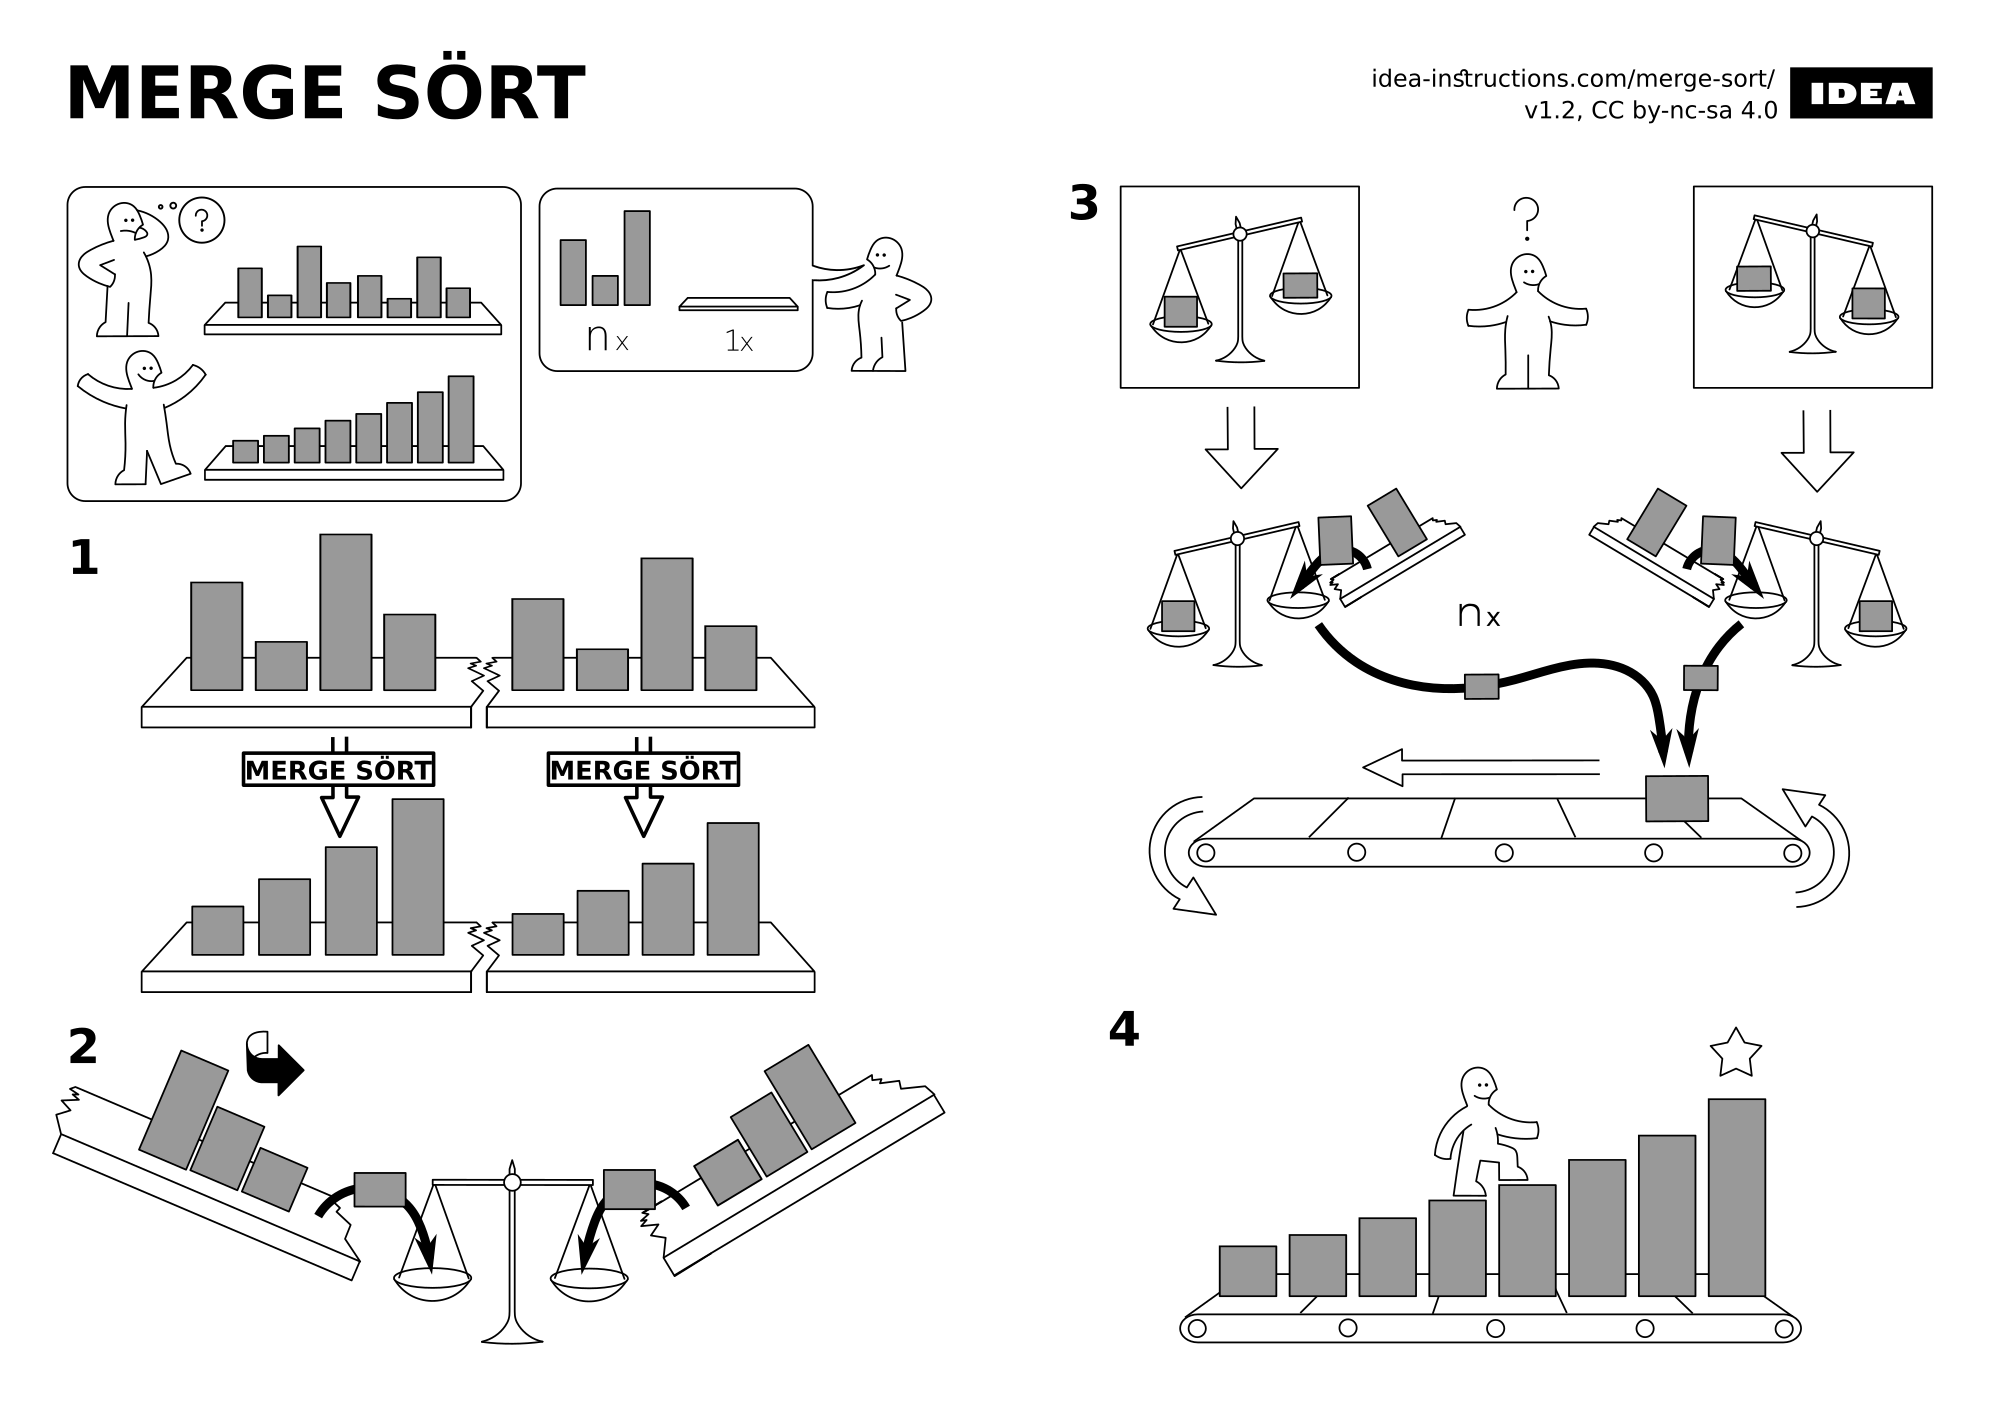
\includegraphics[width=\paperwidth]{merge-sort.png}
      };
    \end{tikzpicture}
  \end{frame}
}

\begin{frame}[plain]
  \begin{center}
    {\huge Programming is a complex intellectual activity that involves modeling}
  \end{center}
\end{frame}

{ % all template changes are local to this group.
  \setbeamertemplate{navigation symbols}{}
  \begin{frame}[plain]
    \begin{tikzpicture}[remember picture,overlay]
      \node[at=(current page.center)] {
        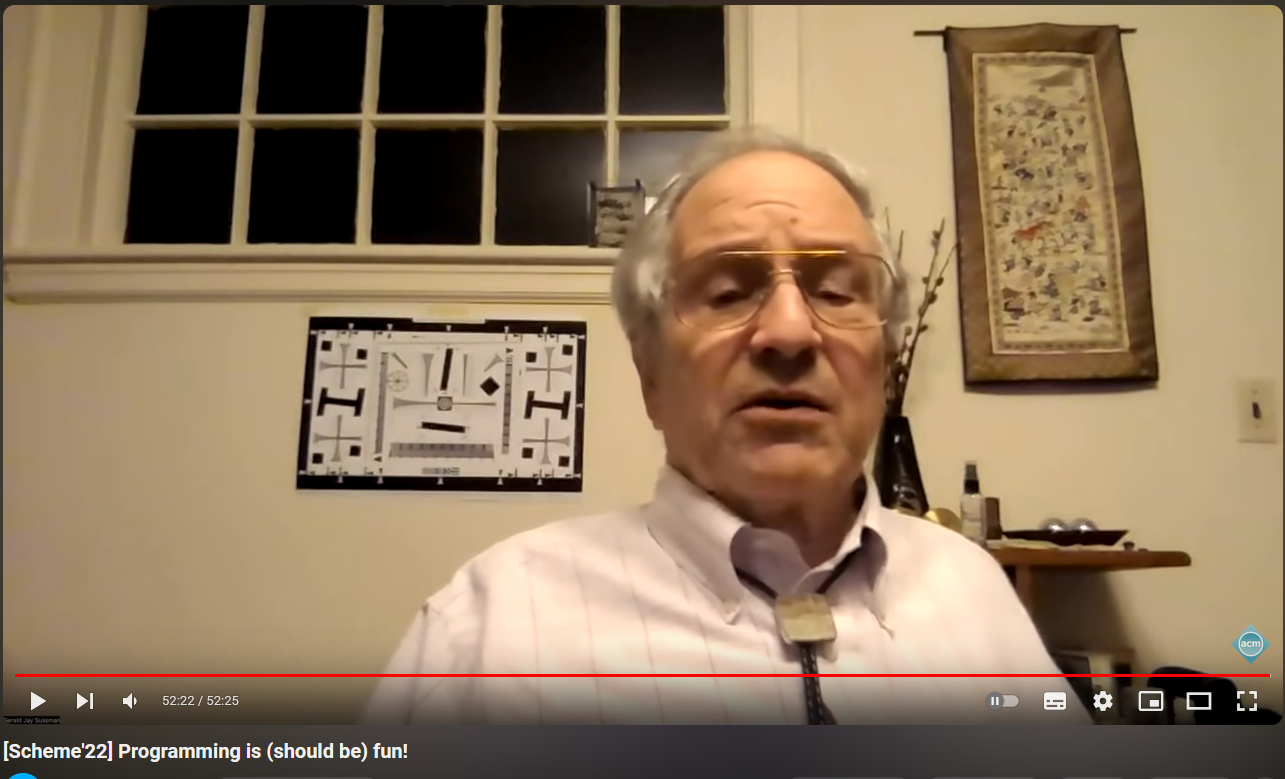
\includegraphics[width=\paperwidth]{sussman.png}
      };
    \end{tikzpicture}
  \end{frame}
}

{ % all template changes are local to this group.
  \setbeamertemplate{navigation symbols}{}
  \begin{frame}[plain]
    \begin{tikzpicture}[remember picture,overlay]
      \node[at=(current page.center)] {
        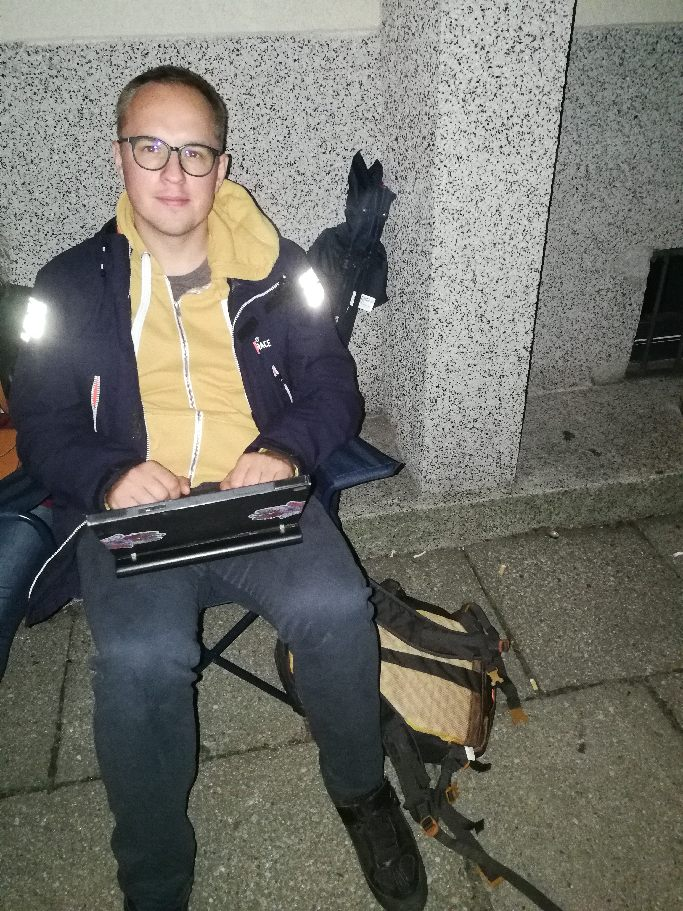
\includegraphics[height=\paperheight]{lato-z-radiem-2018.jpeg}
      };
    \end{tikzpicture}
  \end{frame}
}

{ % all template changes are local to this group.
  \setbeamertemplate{navigation symbols}{}
  \begin{frame}[plain]
    \begin{tikzpicture}[remember picture,overlay]
      \node[at=(current page.center)] {
        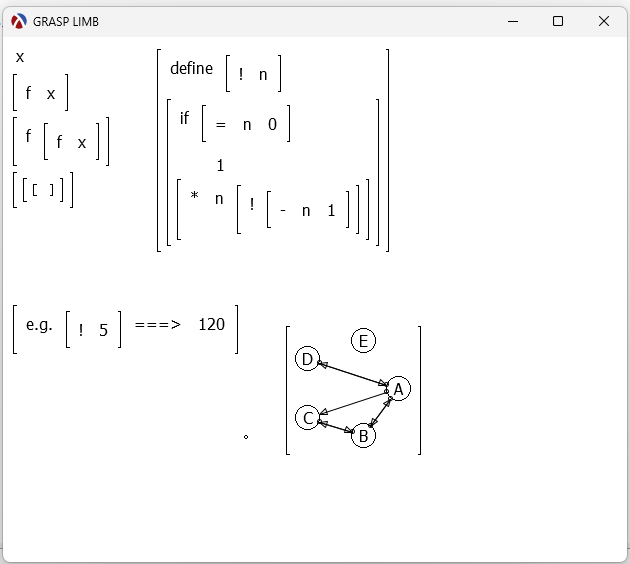
\includegraphics[height=\paperheight]{grasp-limb.png}
      };
    \end{tikzpicture}
  \end{frame}
}

\begin{frame}[plain]
  \null
  {\Large \textit{I want a single piece of glass I can use to read email on the toilet}}
  \\ \null\hfill {\large -- Steve Jobs}
\end{frame}

{ % all template changes are local to this group.
  \setbeamertemplate{navigation symbols}{}
  \begin{frame}[plain]
    \begin{tikzpicture}[remember picture,overlay]
      \node[at=(current page.center)] {
        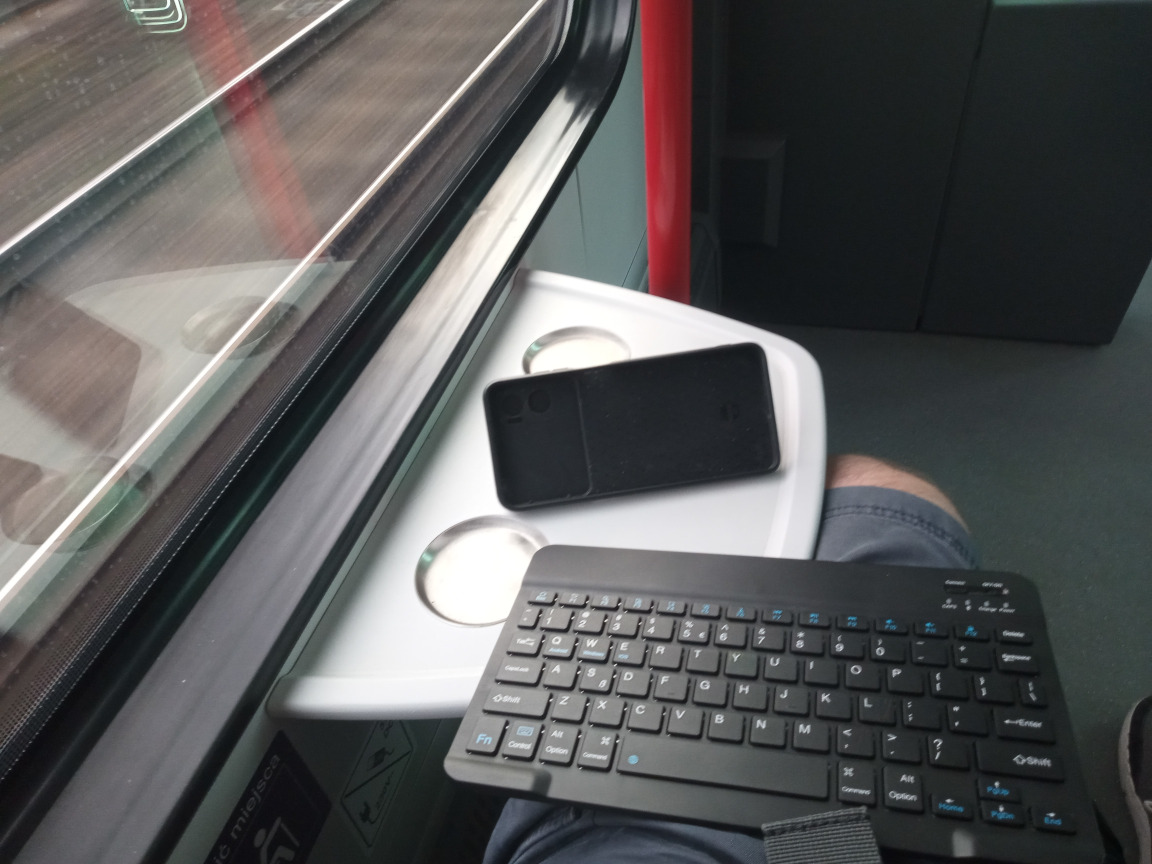
\includegraphics[height=\paperheight]{train-table-phone.jpg}
      };
    \end{tikzpicture}
  \end{frame}
}

{ % all template changes are local to this group.
  \setbeamertemplate{navigation symbols}{}
  \begin{frame}[plain]
    \begin{tikzpicture}[remember picture,overlay]
      \node[at=(current page.center)] {
        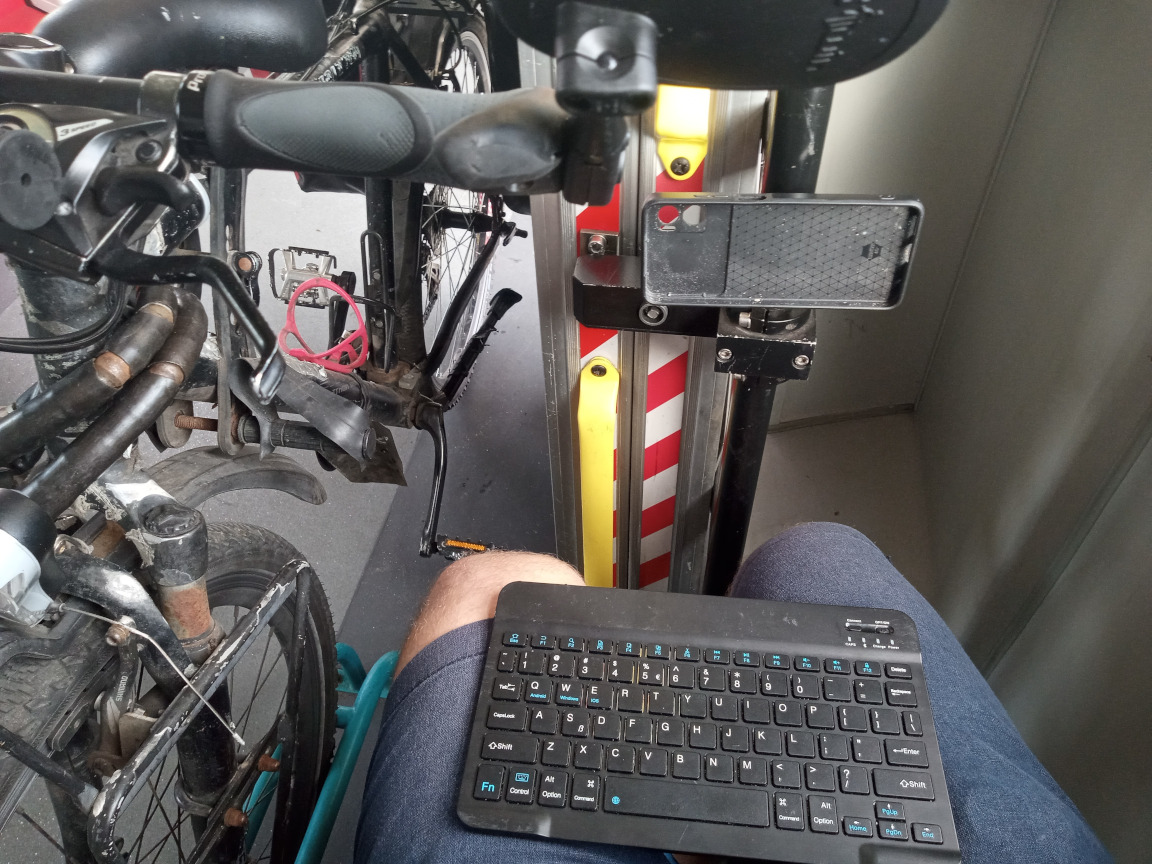
\includegraphics[height=\paperheight]{bike-phone-holder.jpg}
      };
    \end{tikzpicture}
  \end{frame}
}


{ % all template changes are local to this group.
  \setbeamertemplate{navigation symbols}{}
  \begin{frame}[plain]
    \begin{tikzpicture}[remember picture,overlay]
      \node[at=(current page.center)] {
        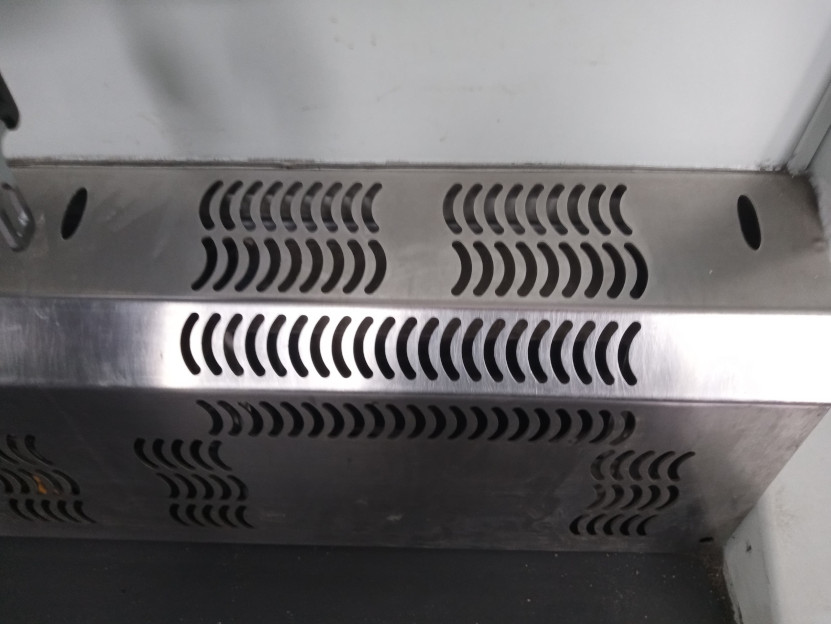
\includegraphics[height=\paperheight]{train-heater.jpg}
      };
    \end{tikzpicture}
  \end{frame}
}

\begin{frame}[plain]
  \begin{center}
    {\tiny GRASP/Java demo}
  \end{center}
\end{frame}

{ % all template changes are local to this group.
  \setbeamertemplate{navigation symbols}{}
  \begin{frame}[plain]
    \begin{tikzpicture}[remember picture,overlay]
      \node[at=(current page.center)] {
        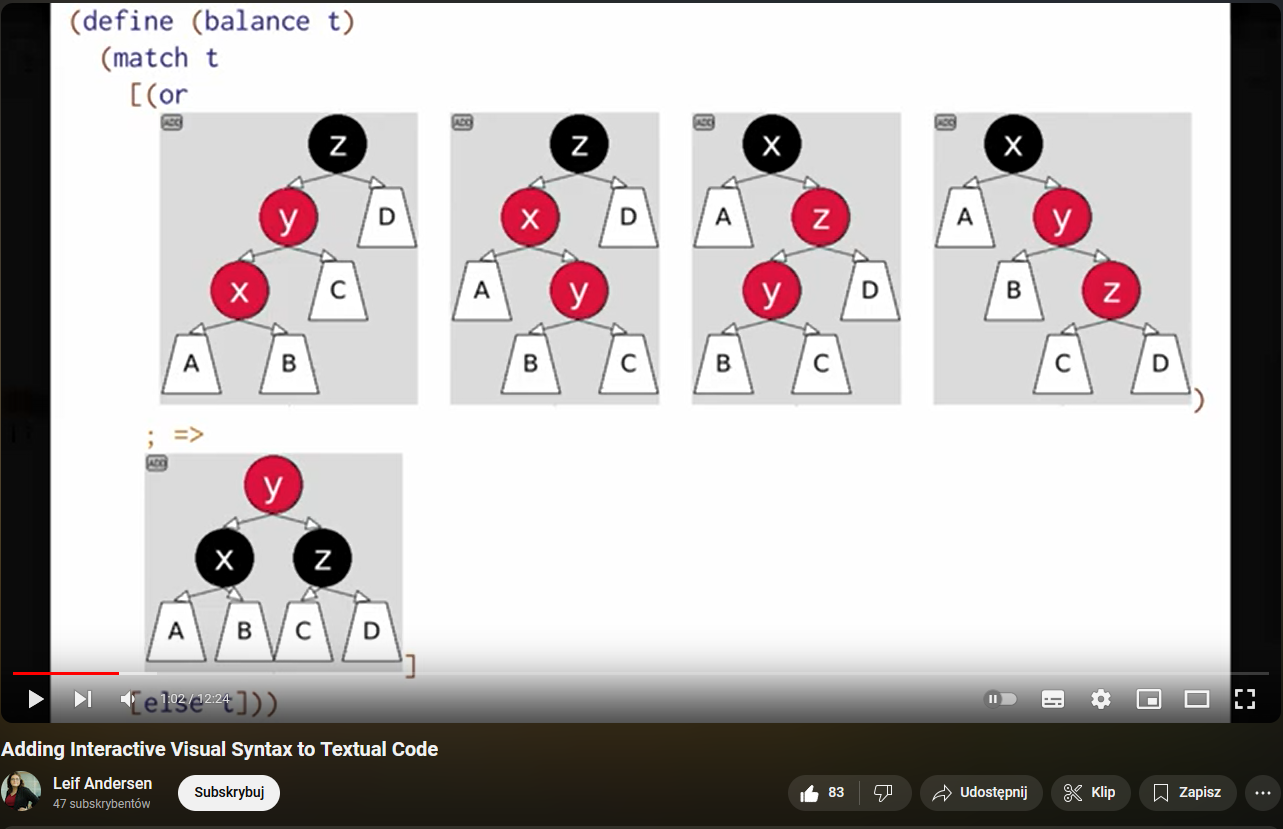
\includegraphics[width=\paperwidth]{leif.png}
      };
    \end{tikzpicture}
  \end{frame}
}

\begin{frame}[plain]
  \begin{center}
    {\tiny GRASP/Kawa demo (stepper)}
  \end{center}
\end{frame}

{ % all template changes are local to this group.
  \setbeamertemplate{navigation symbols}{}
  \begin{frame}[plain]
    \begin{tikzpicture}[remember picture,overlay]
      \node[at=(current page.center)] {
        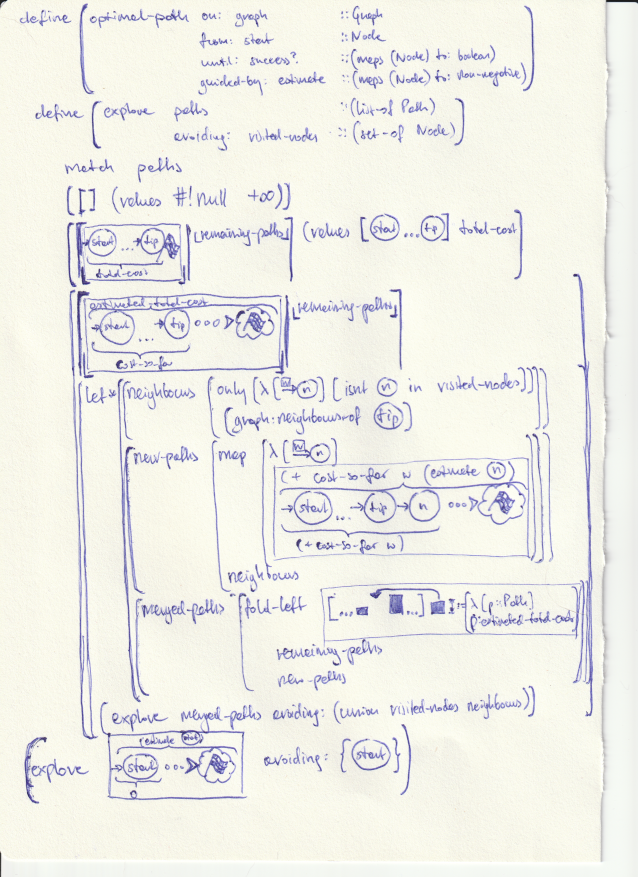
\includegraphics[height=\paperheight]{astar.png}
      };
    \end{tikzpicture}
  \end{frame}
}

{ % all template changes are local to this group.
  \setbeamertemplate{navigation symbols}{}
  \begin{frame}[plain]
    \begin{tikzpicture}[remember picture,overlay]
      \node[at=(current page.center)] {
        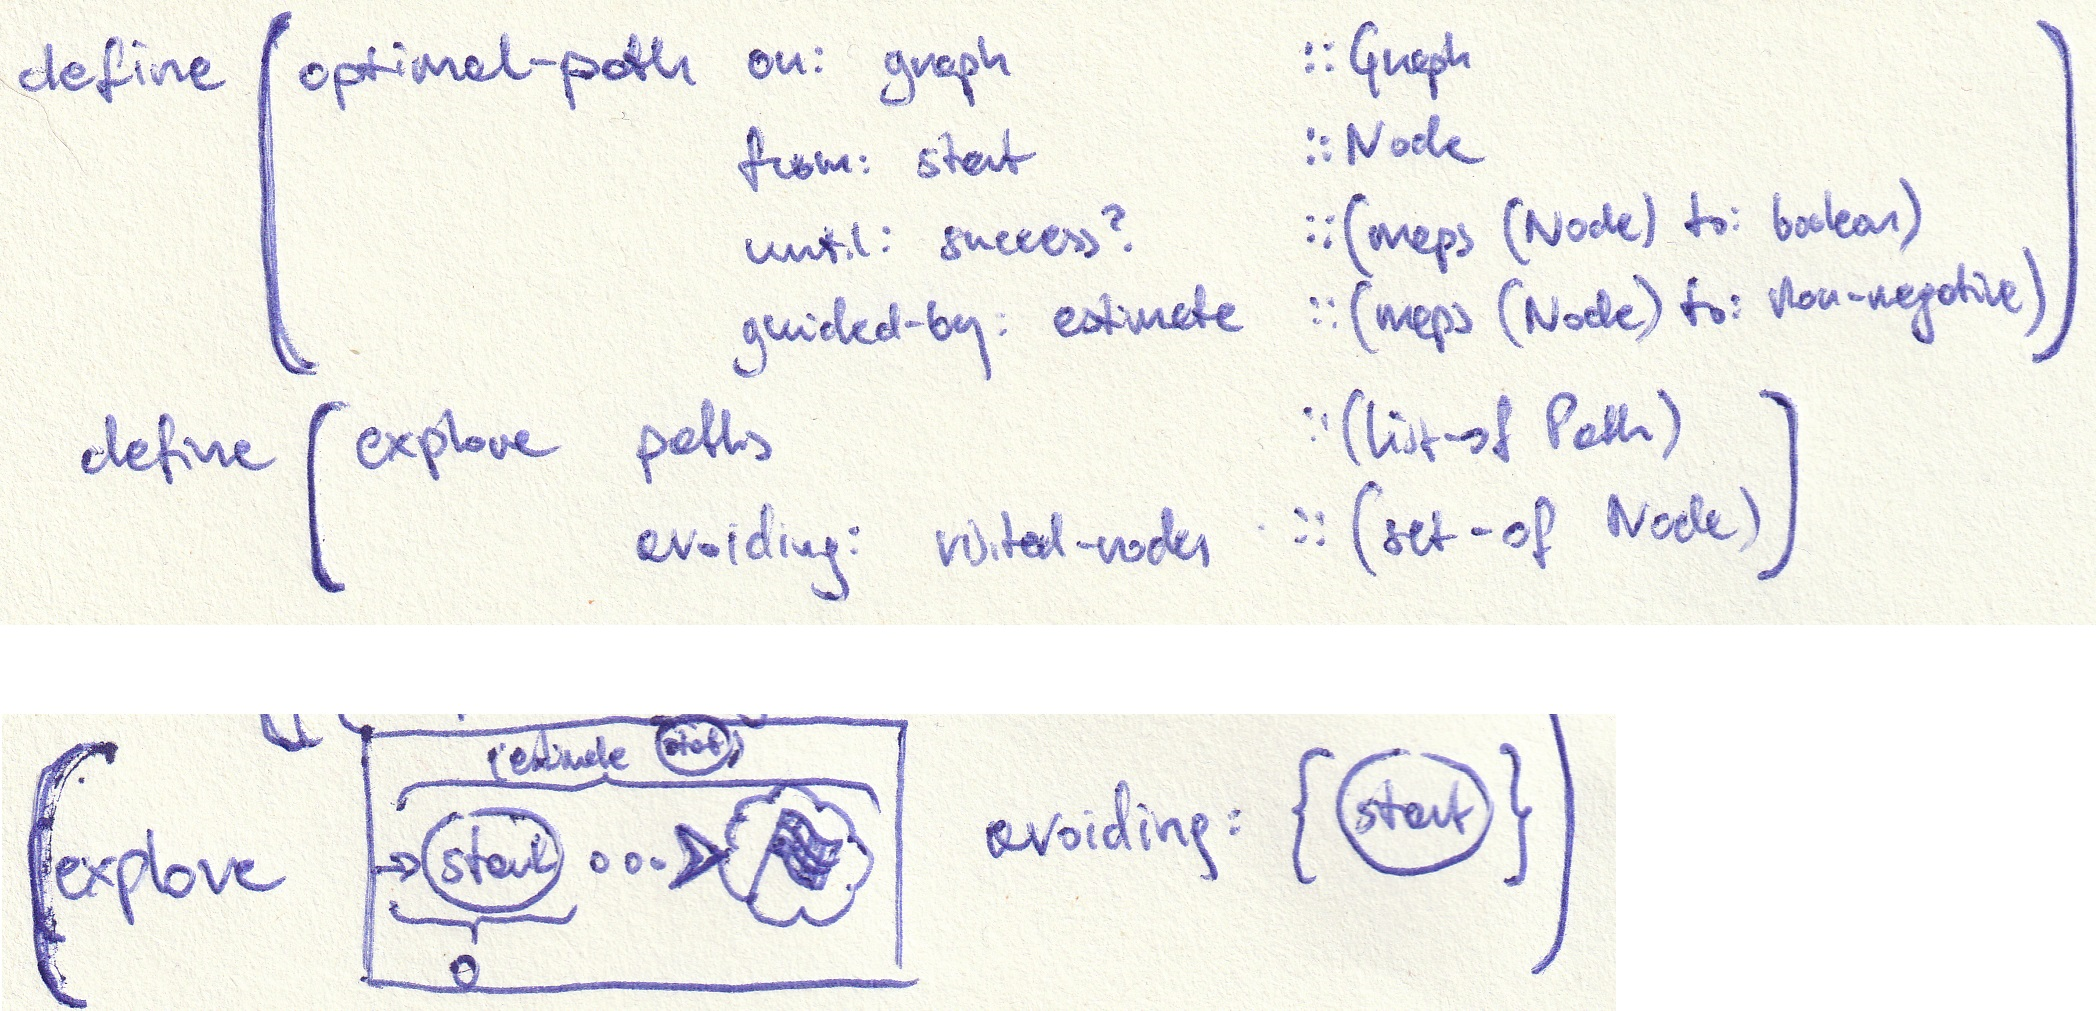
\includegraphics[width=\paperwidth]{astar-sig.jpg}
      };
    \end{tikzpicture}
  \end{frame}
}


{ % all template changes are local to this group.
  \setbeamertemplate{navigation symbols}{}
  \begin{frame}[plain]
    \begin{tikzpicture}[remember picture,overlay]
      \node[at=(current page.center)] {
        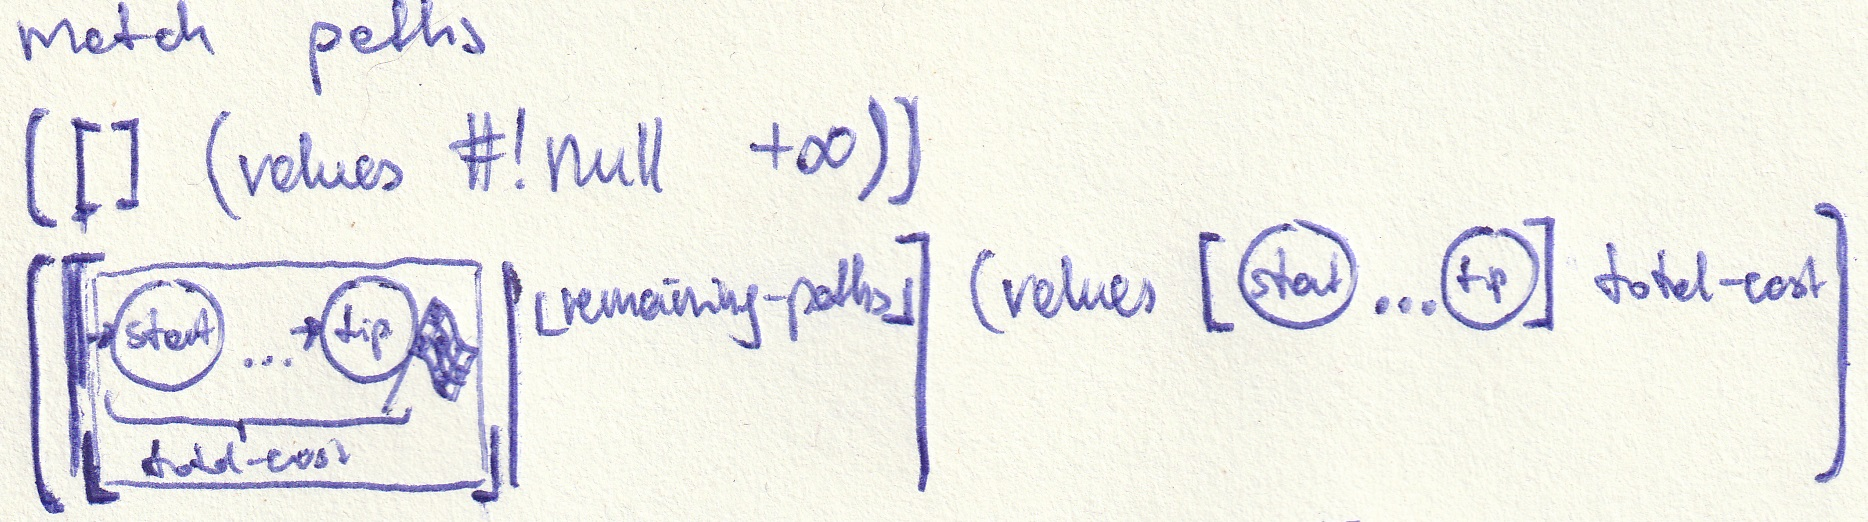
\includegraphics[width=\paperwidth]{astar-case12.jpg}
      };
    \end{tikzpicture}
  \end{frame}
}

{ % all template changes are local to this group.
  \setbeamertemplate{navigation symbols}{}
  \begin{frame}[plain]
    \begin{tikzpicture}[remember picture,overlay]
      \node[at=(current page.center)] {
        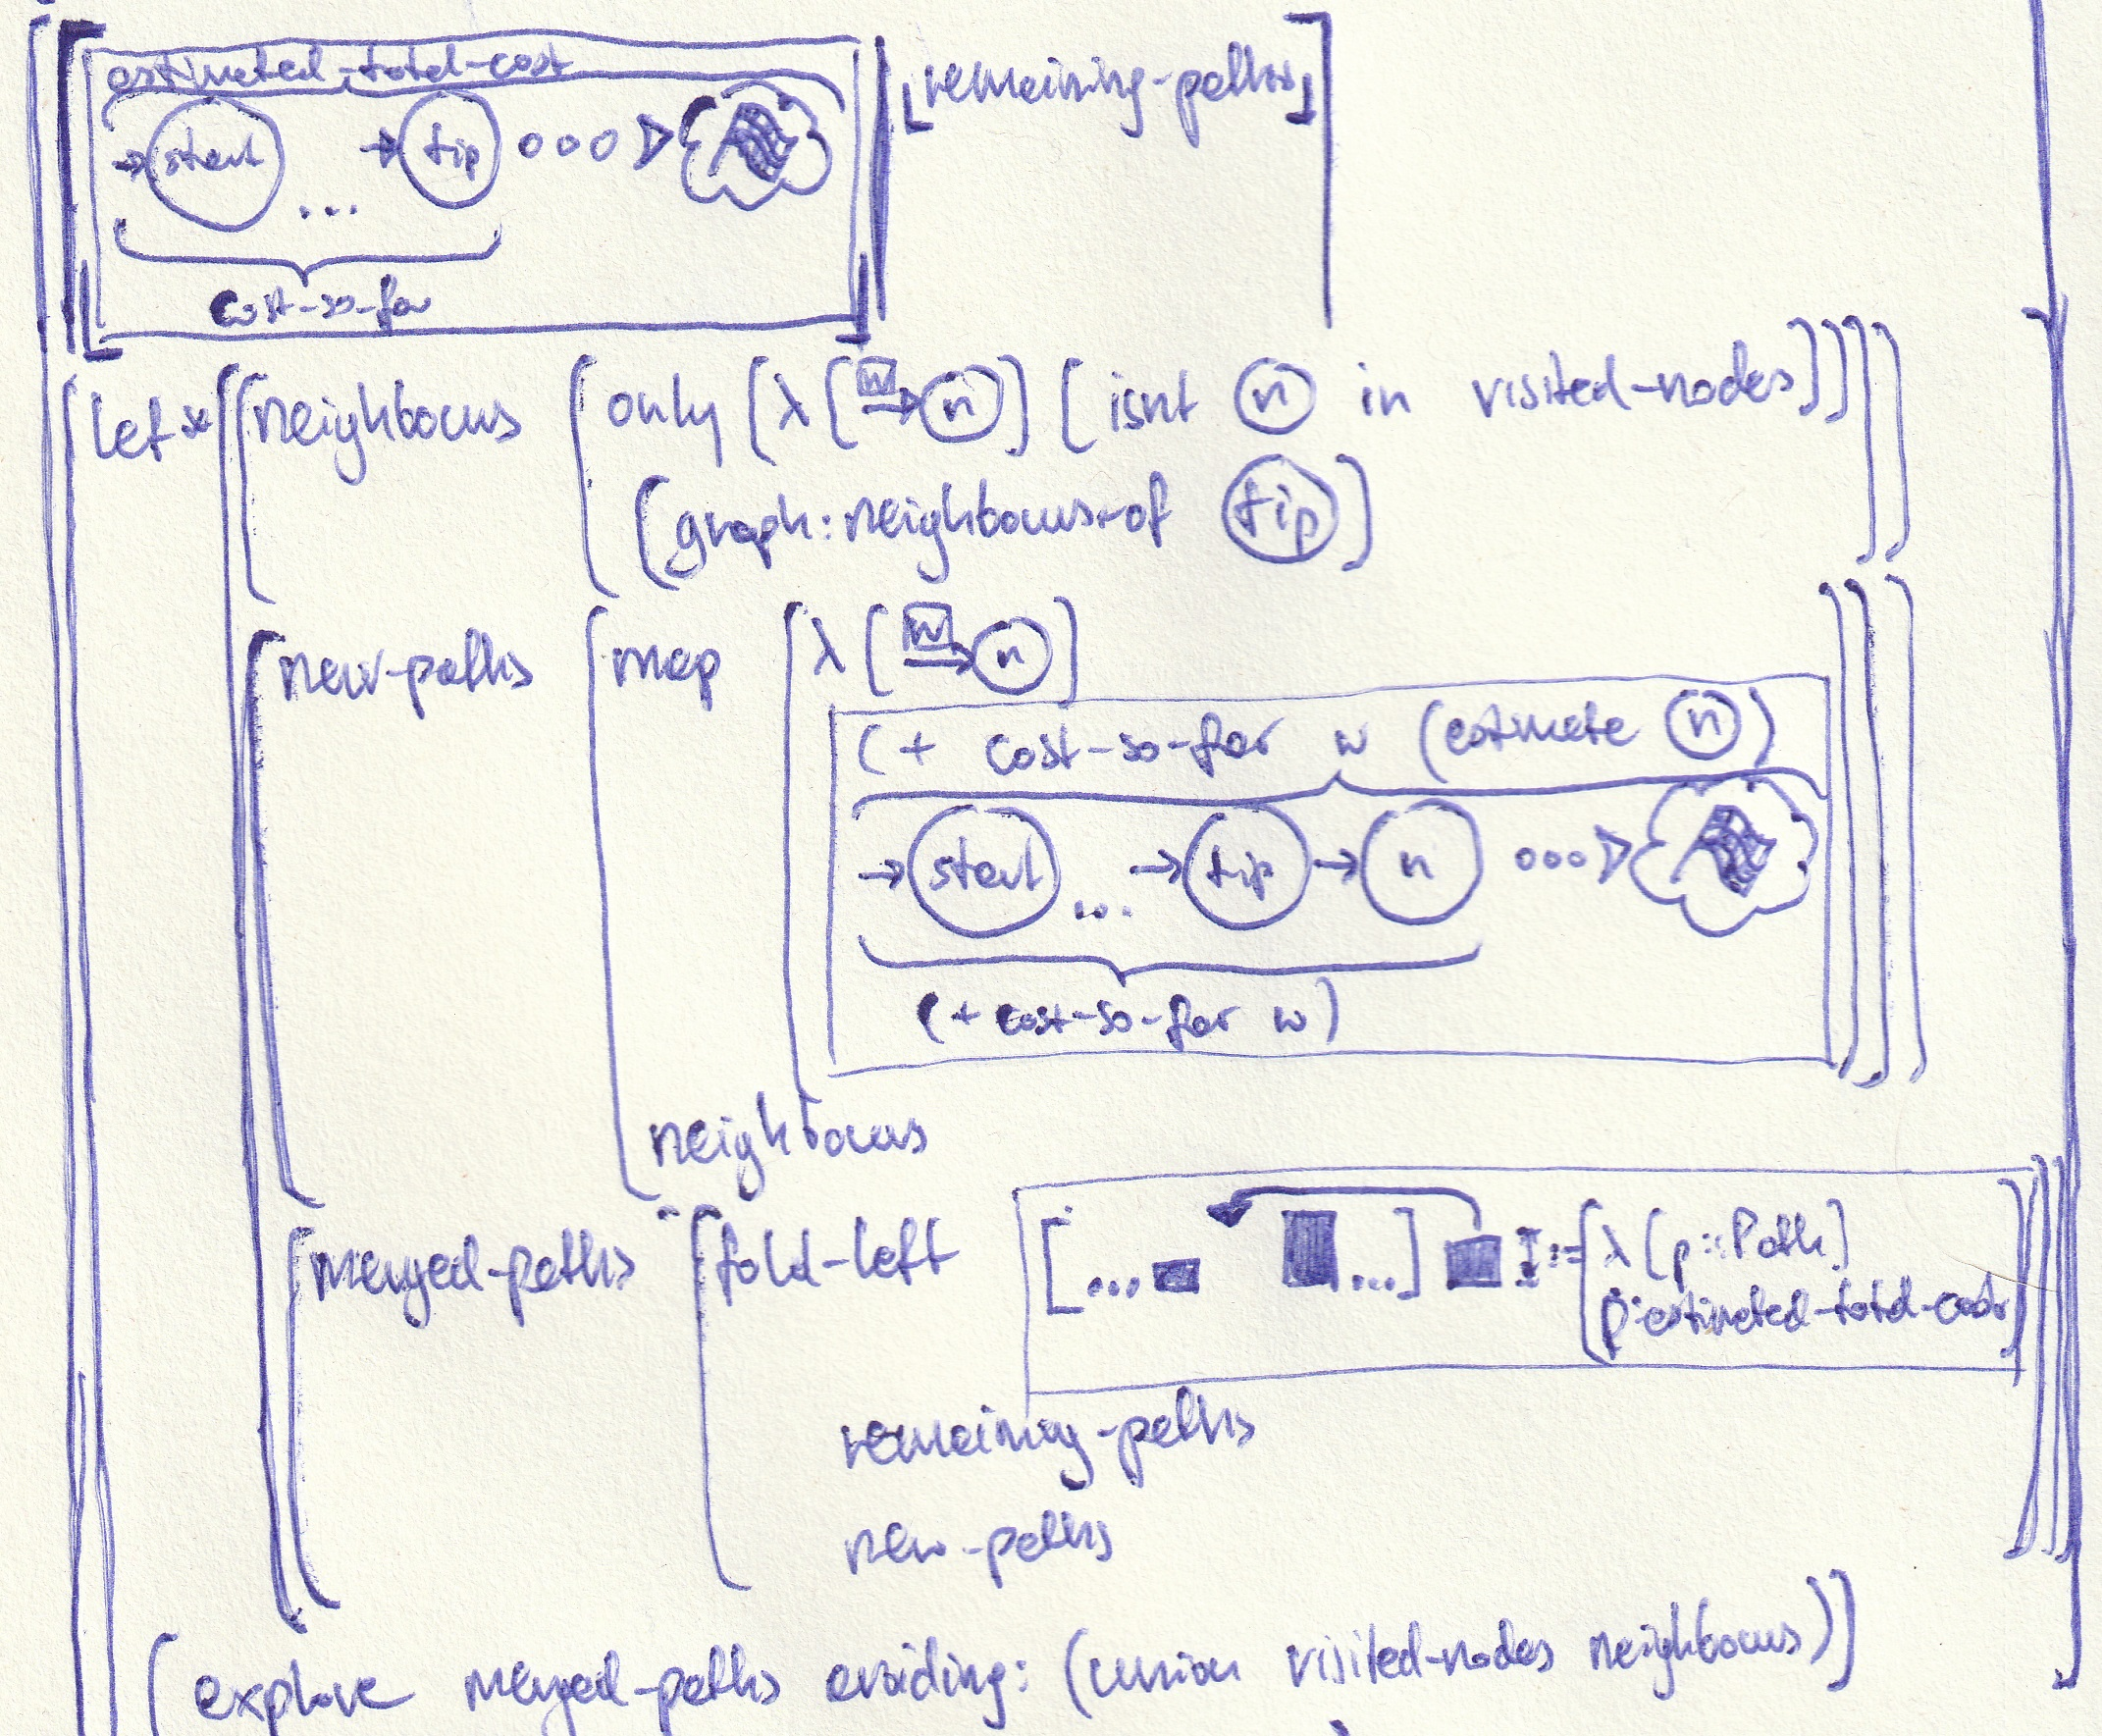
\includegraphics[height=\paperheight]{astar-case3.jpg}
      };
    \end{tikzpicture}
  \end{frame}
}


{ % all template changes are local to this group.
  \setbeamertemplate{navigation symbols}{}
  \begin{frame}[plain]
    \begin{tikzpicture}[remember picture,overlay]
      \node[at=(current page.center)] {
        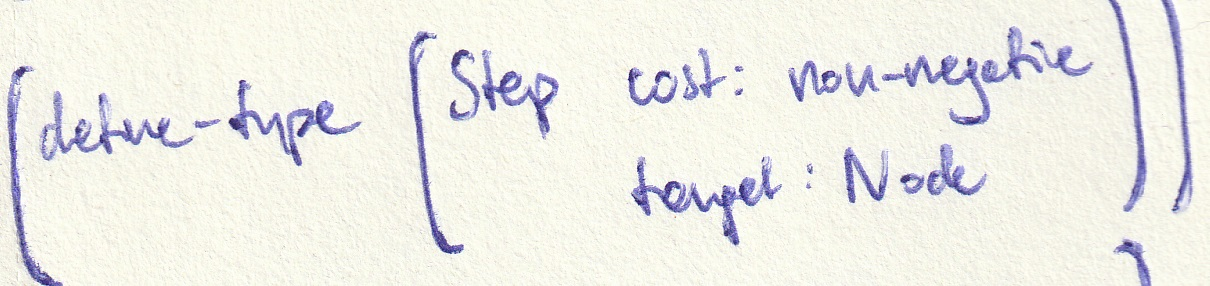
\includegraphics[width=\paperwidth]{step-type.jpg}
      };
    \end{tikzpicture}
  \end{frame}
}

{ % all template changes are local to this group.
  \setbeamertemplate{navigation symbols}{}
  \begin{frame}[plain]
    \begin{tikzpicture}[remember picture,overlay]
      \node[at=(current page.center)] {
        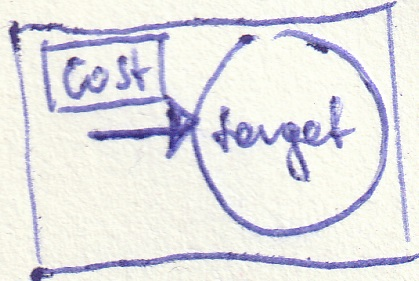
\includegraphics[width=\paperwidth]{step-viz.jpg}
      };
    \end{tikzpicture}
  \end{frame}
}


{ % all template changes are local to this group.
  \setbeamertemplate{navigation symbols}{}
  \begin{frame}[plain]
    \begin{tikzpicture}[remember picture,overlay]
      \node[at=(current page.center)] {
        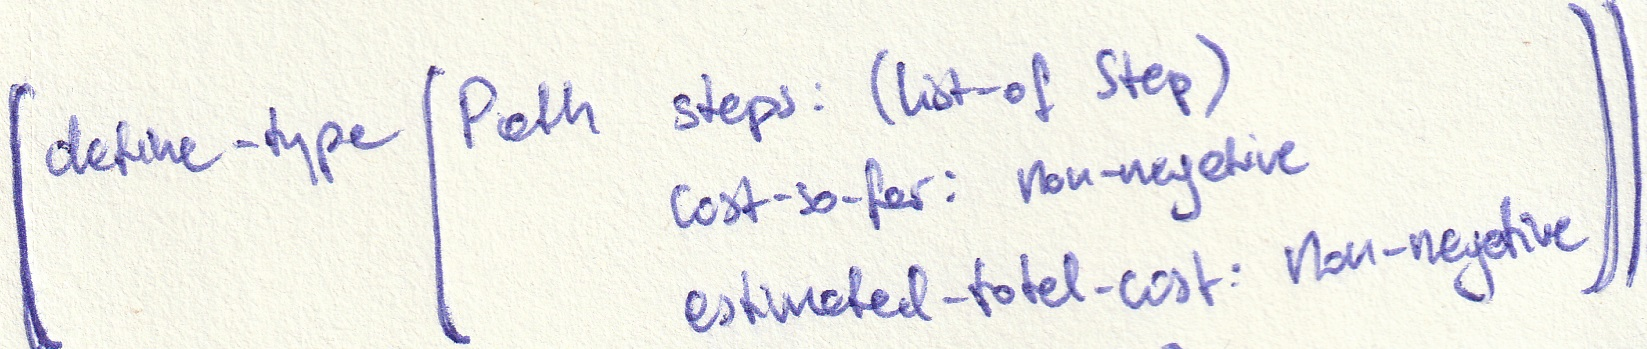
\includegraphics[width=\paperwidth]{path-type.jpg}
      };
    \end{tikzpicture}
  \end{frame}
}

{ % all template changes are local to this group.
  \setbeamertemplate{navigation symbols}{}
  \begin{frame}[plain]
    \begin{tikzpicture}[remember picture,overlay]
      \node[at=(current page.center)] {
        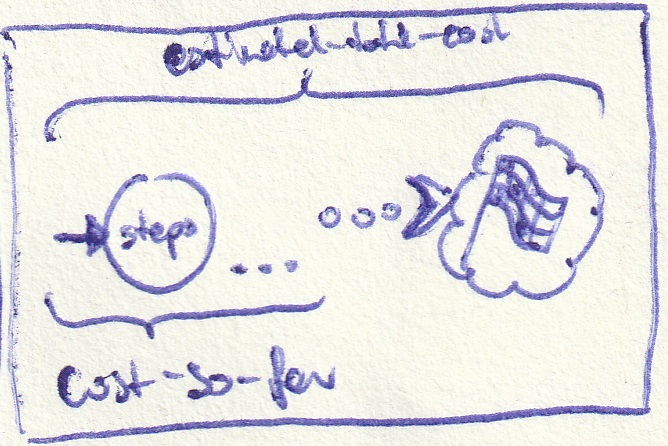
\includegraphics[width=\paperwidth]{path-viz.jpg}
      };
    \end{tikzpicture}
  \end{frame}
}

{ % all template changes are local to this group.
  \setbeamertemplate{navigation symbols}{}
  \begin{frame}[plain]
    \begin{tikzpicture}[remember picture,overlay]
      \node[at=(current page.center)] {
        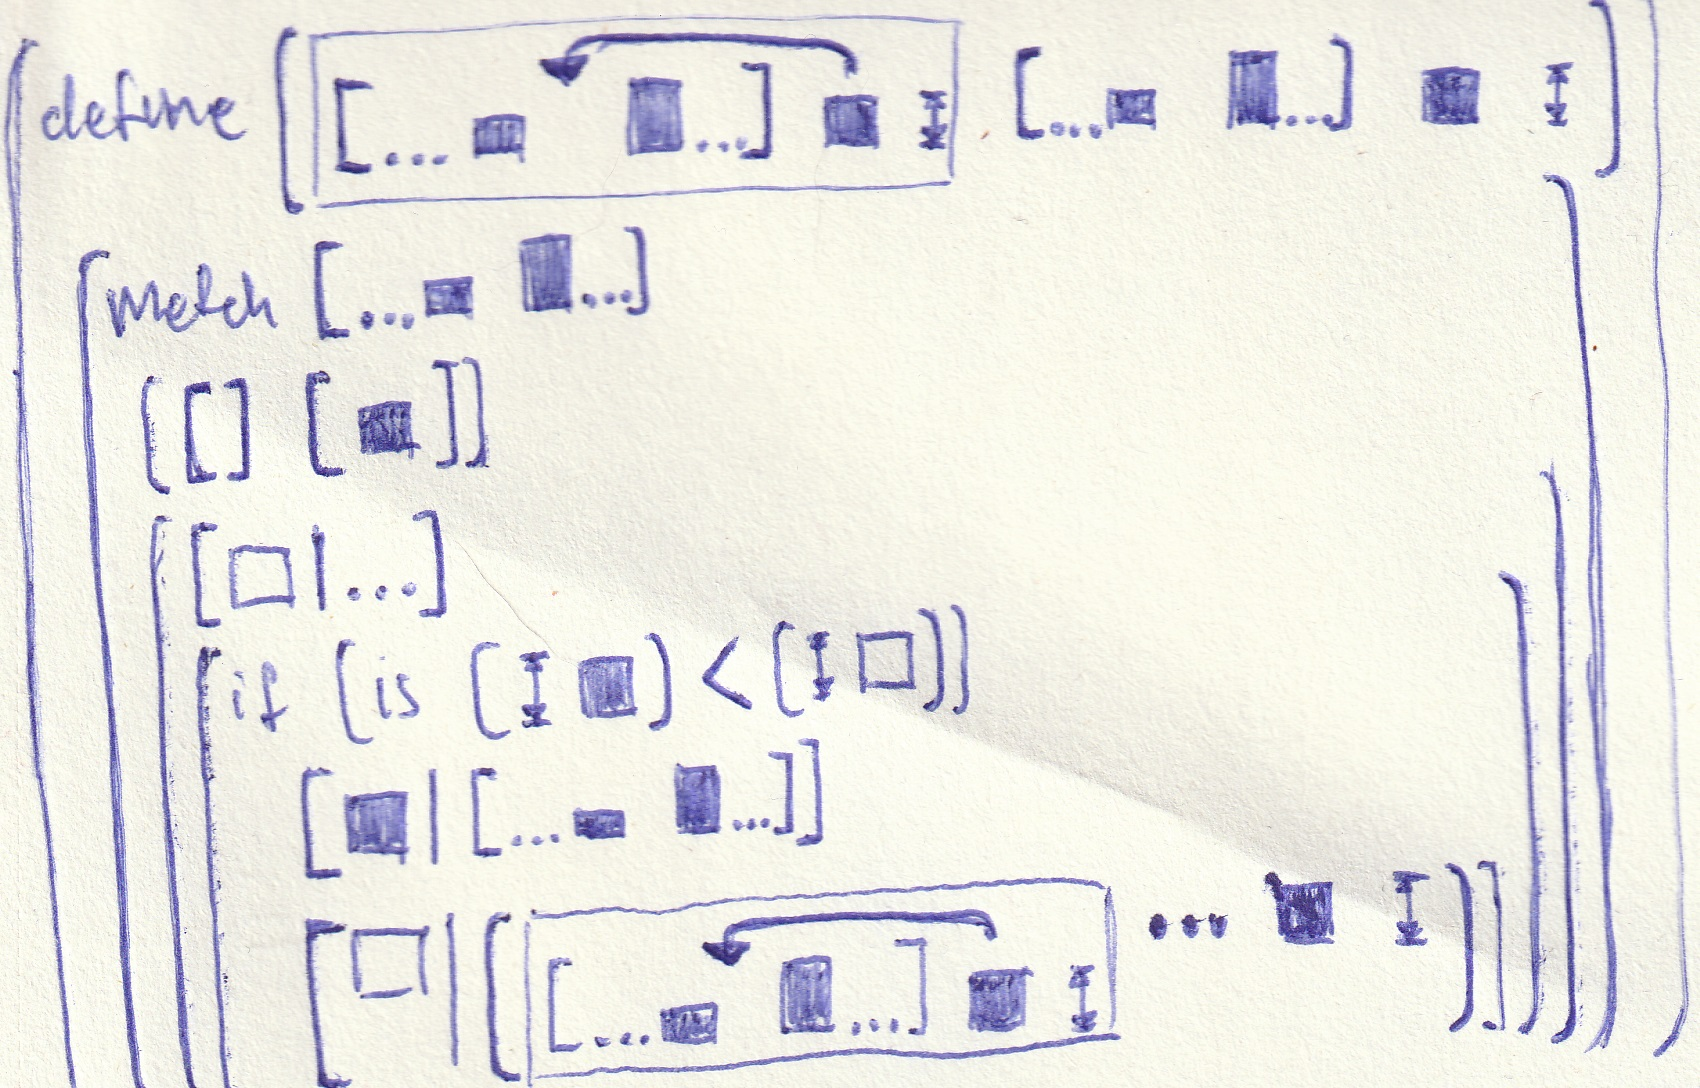
\includegraphics[width=\paperwidth]{merge.png}
      };
    \end{tikzpicture}
  \end{frame}
}

\begin{frame}[plain]
  \begin{center}
    {\tiny GRASP/Kawa demo (zoom out)}
  \end{center}
\end{frame}

{ % all template changes are local to this group.
  \setbeamertemplate{navigation symbols}{}
  \begin{frame}[plain]
    \begin{tikzpicture}[remember picture,overlay]
      \node[at=(current page.center)] {
        
\includegraphics[width=\paperwidth]{toiletpaper.jpg}
      };
    \end{tikzpicture}
  \end{frame}
}

{ % all template changes are local to this group.
  \setbeamertemplate{navigation symbols}{}
  \begin{frame}[plain]
    \begin{tikzpicture}[remember picture,overlay]
      \node[at=(current page.center)] {
        
\includegraphics[height=\paperheight]{is-this-architecture-diagram.png}
      };
    \end{tikzpicture}
  \end{frame}
}


{ % all template changes are local to this group.
  \setbeamertemplate{navigation symbols}{}
  \begin{frame}[plain]
    \begin{tikzpicture}[remember picture,overlay]
      \node[at=(current page.center)] {
        
\includegraphics[width=\paperwidth]{rethinking.png}
      };
    \end{tikzpicture}
  \end{frame}
}


{ % all template changes are local to this group.
  \setbeamertemplate{navigation symbols}{}
  \begin{frame}[plain]
    \begin{tikzpicture}[remember picture,overlay]
      \node[at=(current page.center)] {
        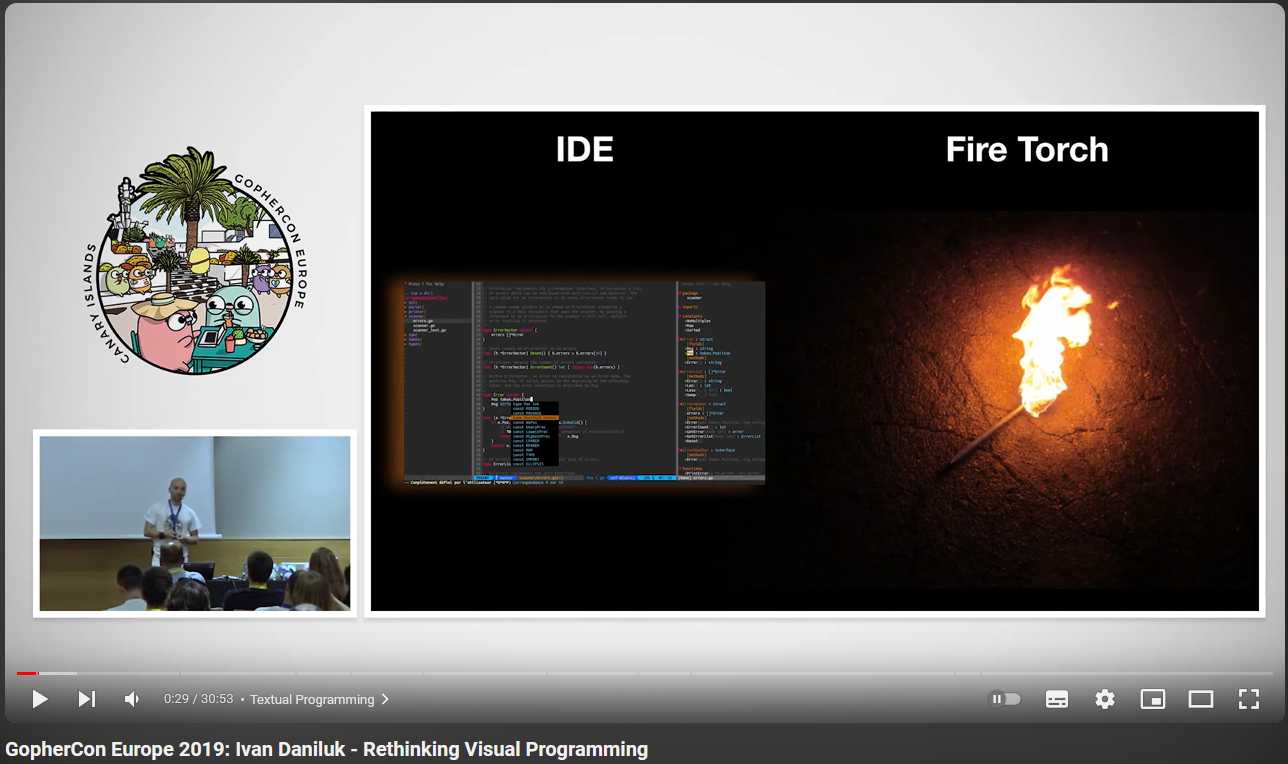
\includegraphics[width=\paperwidth]{torch.png}
      };
    \end{tikzpicture}
  \end{frame}
}

{ % all template changes are local to this group.
  \setbeamertemplate{navigation symbols}{}
  \begin{frame}[plain]
    \begin{tikzpicture}[remember picture,overlay]
      \node[at=(current page.center)] {
        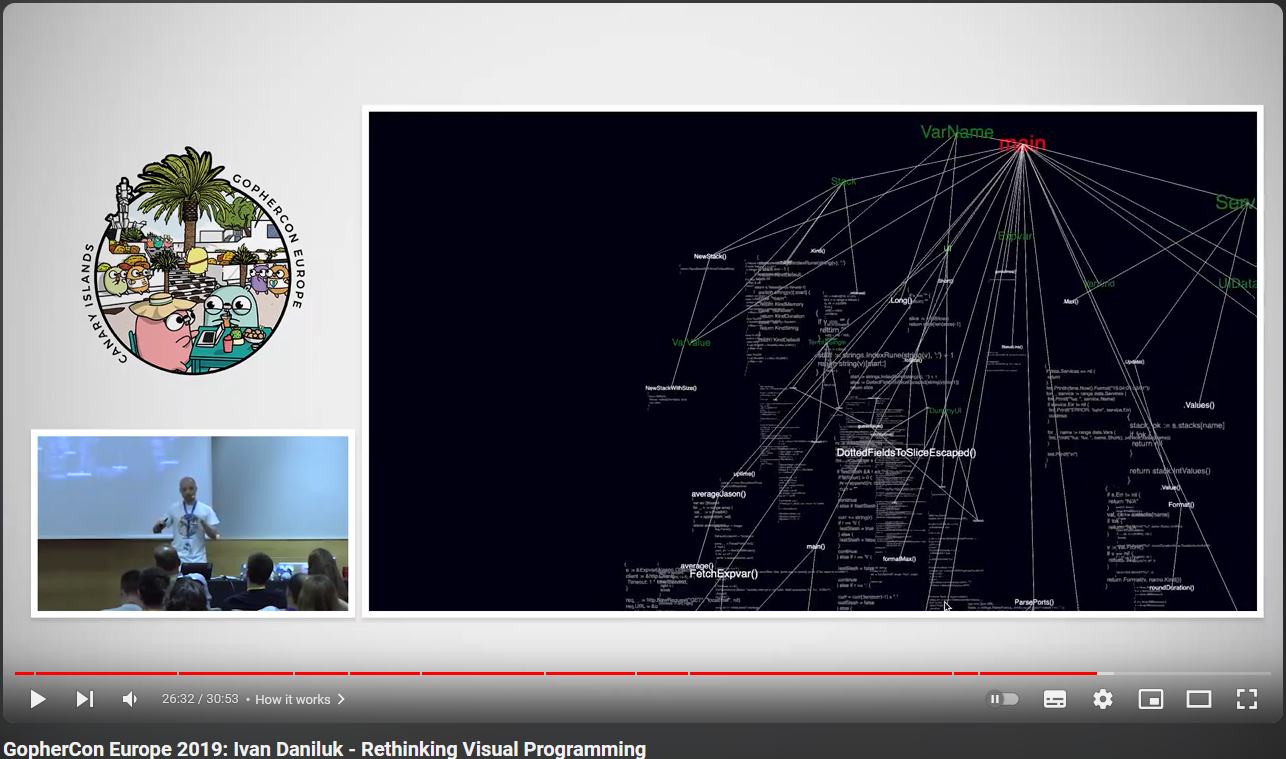
\includegraphics[width=\paperwidth]{3dgraph.png}
      };
    \end{tikzpicture}
  \end{frame}
}

{ % all template changes are local to this group.
  \setbeamertemplate{navigation symbols}{}
  \begin{frame}[plain]
    \begin{tikzpicture}[remember picture,overlay]
      \node[at=(current page.center)] {
        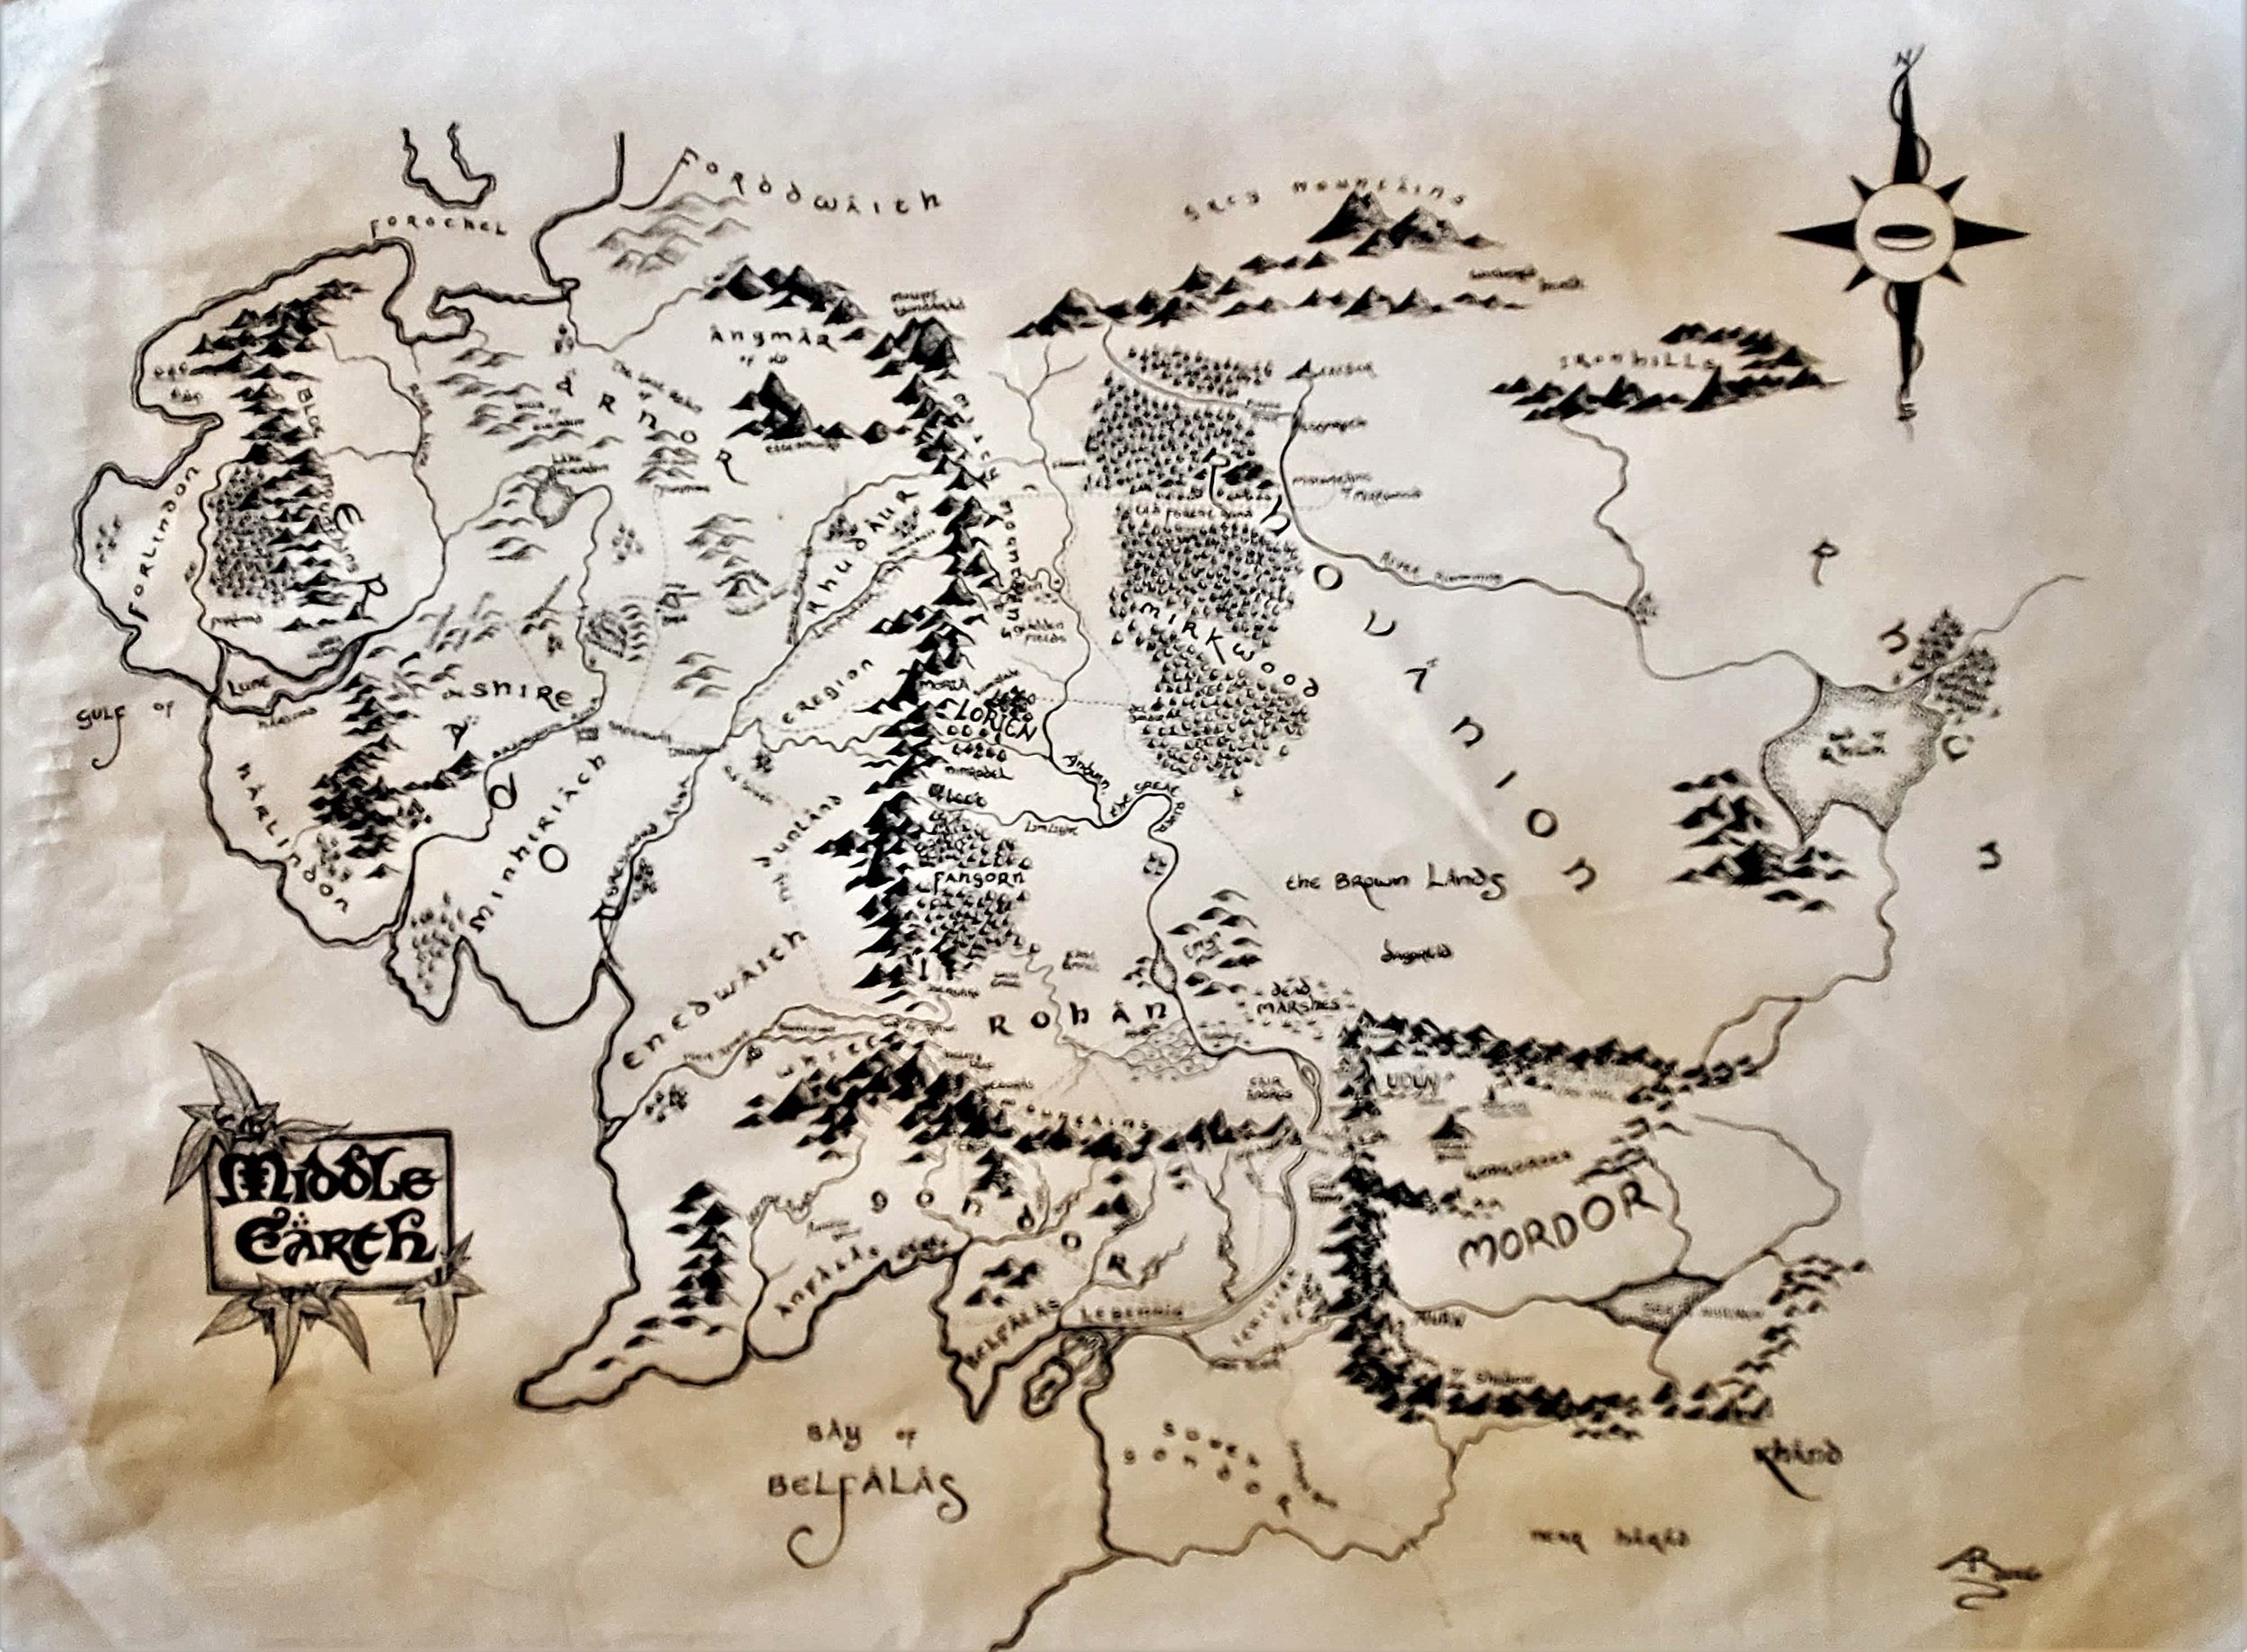
\includegraphics[width=\paperwidth]{middle-earth.jpg}
      };
    \end{tikzpicture}
  \end{frame}
}


{ % all template changes are local to this group.
  \setbeamertemplate{navigation symbols}{}
  \begin{frame}[plain]
    \begin{tikzpicture}[remember picture,overlay]
      \node[at=(current page.center)] {
        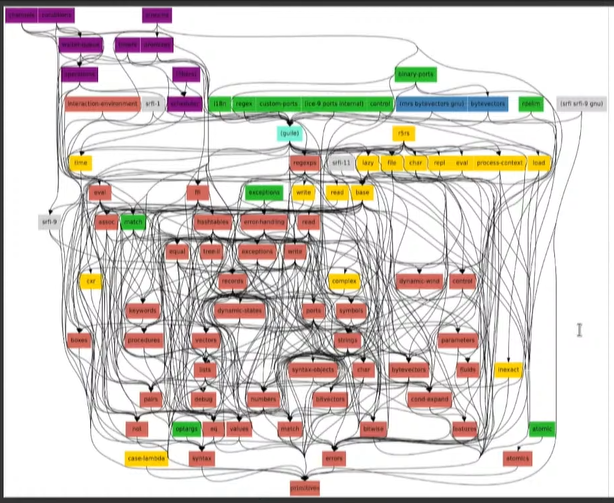
\includegraphics[width=\paperwidth]{module-graph.png}
      };
    \end{tikzpicture}
  \end{frame}
}


\begin{frame}[plain]
  So, I want my code editor to
  \begin{itemize}
    \item be pleasant to use on the phone
    \item support interactive visual syntax
    \item provide abstract code view and a module browser
  \end{itemize}
\end{frame}


\end{document}
